\documentclass{plt}

\title{Names, Scope, and Types}
\author{Stephen A. Edwards}
\institute{Columbia University}
\date{Fall 2018}
\titlegraphic{
\includegraphics[height=6pc]{nametag.jpg}\quad
\includegraphics[height=6pc]{telescope.jpg}\quad
\includegraphics[height=6pc]{typewriter.jpg}
}

\usetikzlibrary{shapes.geometric}

\begin{document}

\frame{\titlepage}

\frame{\tableofcontents}

\begin{frame}{What's Wrong With This?}

\centerline{\Huge \texttt{a + f(b, c)}}

\pause

\begin{center}
\color{red}
Is \texttt{a} defined?

Is \texttt{f} defined?

Are \texttt{b} and \texttt{c} defined?

\color{blue}
Is \texttt{f} a function of two arguments?

Can you add whatever \texttt{a} is to whatever \texttt{f} returns?

Does \texttt{f} accept whatever \texttt{b} and \texttt{c} are?

\medskip

\color{red} Scope questions \quad \color{blue} Type questions
\end{center}

\end{frame}

\part{Scope}
\frame{\partpage

\centerline{What names are visible?}

\centerline{\includegraphics[width=0.35\textwidth]{telescope.jpg}}
}

\begin{frame}

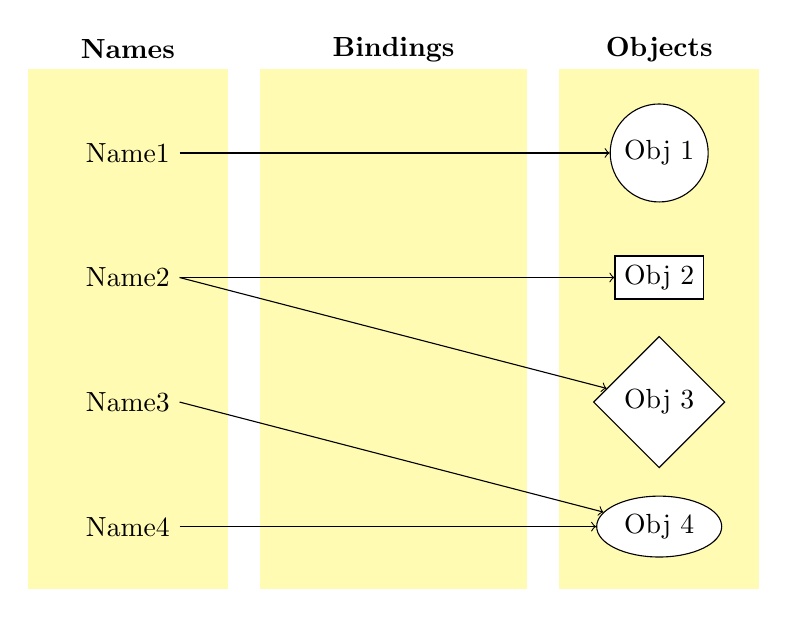
\begin{tikzpicture}[x=4pc,y=2.5pc,node distance=1.6pc]
\draw [fill,color=yellow!30]
   (-0.75,-0.75) rectangle ++(1.5,6.25)
   ++(right:0.25) rectangle ++(2,-6.25)
   ++(right:0.25) rectangle ++(1.5,6.25);
\node at (0,5.75) {\textbf{Names}};
\node at (2,5.75) {\textbf{Bindings}};
\node at (4,5.75) {\textbf{Objects}};
  \begin{scope}[every node/.style={draw,fill=white}]
    \node [circle] at (4,4.5) (obj1) {Obj 1};
    \node at (4,3) (obj2) {Obj 2};
    \node [diamond] at (4,1.5) (obj3) {Obj 3};
    \node [ellipse] at (4,0) (obj4) {Obj 4};
  \end{scope}

  \node at (0,4.5) (name1) {Name1};
  \node at (0,3) (name2) {Name2};
  \node at (0,1.5) (name3) {Name3};
  \node at (0,0) (name4) {Name4};

  \begin{scope}[every path/.style={draw,->}]
    \path (name1.east) -- (obj1);
    \path (name2.east) -- (obj2);
    \path (name2.east) -- (obj3);
    \path (name3.east) -- (obj4);
    \path (name4.east) -- (obj4);
  \end{scope}
\end{tikzpicture}

\end{frame}

\begin{frame}{Scope}

Scope: where/when a name is bound to an object

Useful for modularity: want to keep most things hidden

\medskip

\begin{center}
\begin{tabular}{ll}
\toprule
\textbf{Scoping} & \textbf{Visible Names Depend On} \\
\textbf{Policy} \\
\midrule
Static & Textual structure of program \\
  & Names resolved by compile-time symbol tables \\
  & Faster, more common \\
\\
Dynamic & Run-time behavior of program \\
  & Names resolved by run-time symbol tables,\\
  & e.g., walk the stack looking for names \\
  & Slower, more dynamic \\
\bottomrule
\end{tabular}
\end{center}

\end{frame}


\begin{frame}[fragile]{Basic Static Scope in C, C++, Java, etc.}
  \begin{columns}
    \begin{column}{0.5\textwidth}
\parskip=1pc

A name begins life where it is declared and ends at the end
of its block.

From the CLRM, ``The scope of an identifier declared at the head of a
block begins at the end of its declarator, and persists to the end of
the block.''
    \end{column}
    \begin{column}{0.5\textwidth}
\begin{showscope}
void foo()
\{
   int x;[                 ]
[                          ]
[                          ]
[                          ]
\}%
\end{showscope}
    \end{column}
  \end{columns}
\end{frame}

\begin{frame}[fragile]{Hiding a Definition}

  \begin{columns}
    \begin{column}{0.5\textwidth}
\parskip=1pc
Nested scopes can hide earlier definitions, giving a hole.

From the CLRM, ``If an identifier is explicitly declared at the head
of a block, including the block constituting a function, any
declaration of the identifier outside the block is suspended until the
end of the block.''
    \end{column}
    \begin{column}{0.5\textwidth}
\begin{showscope}
void foo()
\{
  int x;[                  ]
[                          ]
[  while ( a < 10 ) ]\{      
    int x;

  \}[                       ]
[                          ]
[                          ]
\}%
\end{showscope}
    \end{column}
  \end{columns}
\end{frame}

\begin{frame}[fragile]{Static vs. Dynamic Scope}

\begin{columns}[t]
\begin{column}{0.3\textwidth}
\centerline{C}

\vspace{0.5\baselineskip}

\begin{C}
int a = 0;

int foo() {
  return a + 1;
}

int bar() {
  int a = 10;

  return foo();
}
\end{C}
\end{column}
\begin{column}{0.3\textwidth}
\centerline{OCaml}

\vspace{0.5\baselineskip}

\begin{ocaml}
let a = 0 in
let foo x = a + 1 in
let bar =
  let a = 10 in
  foo 0
\end{ocaml}
\end{column}
\begin{column}{0.3\textwidth}
\centerline{Bash}

\vspace{0.5\baselineskip}

\begin{bash}
a=0

foo ()
{
  a=`expr $a + 1`
}

bar ()
{
  local a=10
  foo
  echo $a
}

bar
\end{bash}
% 1 under static scoping (C, OCaml)
% 11 under dynamic (Bash)
\end{column}
\end{columns}

\end{frame}

\begin{frame}[fragile]{Basic Static Scope in O'Caml}
  \begin{columns}
    \begin{column}{0.5\textwidth}
A name is bound after the ``in'' clause of a ``let.''  If the name is
re-bound, the binding takes effect \emph{after} the ``in.''
    \end{column}
    \begin{column}{0.5\textwidth}
\begin{showscope}
let x = 8 in [             ]
[                          ]
[                          ]
let x = [x + 1] in

\end{showscope}

Returns the pair (12, 8):

\begin{showscope}
let x = 8 in[              ]
[  ](let x = [ x + 2 ]in
    x + 2),[               ]
[x                         ]%
\end{showscope}

    \end{column}
  \end{columns}
\end{frame}

\begin{frame}[fragile]{Let Rec in O'Caml}
  \begin{columns}
    \begin{column}{0.5\textwidth}
The ``rec'' keyword makes a name visible to its definition.  This only
makes sense for functions.
    \end{column}
    \begin{column}{0.5\textwidth}
\begin{showscope}
let rec fib i =[           ]
[  if i < 1 then 1 else    ]
[    fib (i-1) + fib (i-2) ]
[in                        ]
[  fib 5]%
\end{showscope}

\begin{showscope}
(* Nonsensical *)
let rec x =[ x + 3 in      ]
[                          ]
\end{showscope}
    \end{column}
  \end{columns}
\end{frame}

\begin{frame}[fragile]{Let...and in O'Caml}

  \begin{columns}
    \begin{column}{0.5\textwidth}
Let...and lets you bind multiple names at once.  Definitions are not
mutually visible unless marked ``rec.''
    \end{column}
    \begin{column}{0.5\textwidth}
\begin{showscope}
let x = 8
and y = 9 in
[                          ]
[                          ]
\end{showscope}
\begin{showscope}
let rec fac n = [          ]
[     if n < 2 then        ]
[       1                  ]
[     else                 ]
[       n * fac1 n         ]
and fac1 n = [fac (n - 1)  ]
in
[fac 5]%
\end{showscope}
    \end{column}
  \end{columns}
\end{frame}

\begin{frame}[fragile]{Forward Declarations}

Languages such as C, C++, and Pascal require \emph{forward
declarations} for mutually-recursive references.

\begin{C}
int foo(void);
int bar() { ... foo(); ... }
int foo() { ... bar(); ... }
\end{C}

Partial side-effect of compiler implementations.  Allows single-pass
compilation.

\end{frame}

\begin{frame}[fragile]{Dynamic Definitions in \TeX}

\begin{tex}
% \x, \y undefined
{
  % \x, \y undefined
  \def \x 1
  % \x defined, \y undefined

  \ifnum \a < 5
    \def \y 2
  \fi

  % \x defined, \y may be undefined
}
% \x, \y undefined
\end{tex}

\end{frame}

\begin{frame}{Static vs. Dynamic Scope}

Most modern languages use static scoping.

Easier to understand, harder to break programs.

Advantage of dynamic scoping: ability to change environment.

A way to surreptitiously pass additional parameters.

\end{frame}

\begin{frame}[fragile]{Application of Dynamic Scoping}

\begin{pascal}
program messages;
var message : string;

  procedure complain;
  begin
    writeln(message);
  end

  procedure problem1;
  var message : string;
  begin
    message := 'Out of memory';
    complain 
  end

  procedure problem2;
  var message : string;
  begin
    message := 'Out of time';
    complain
  end
\end{pascal}

\end{frame}

\begin{frame}[fragile]{Open vs. Closed Scopes}

An \emph{open scope} begins life including the symbols in its outer
scope.

Example: blocks in Java

\begin{java}
{
  int x;
  for (;;) {
    /* x visible here */
  }
}
\end{java}

A \emph{closed scope} begins life devoid of symbols.

Example: structures in C.

\begin{C}
struct foo {
  int x;
  float y;
}
\end{C}

\end{frame}

\part{Types}
\frame{\partpage

\centerline{What operations are allowed?}

\centerline{\includegraphics[width=0.35\textwidth]{square-peg-round-hole.jpg}}
}

\begin{frame}{Types}

\emph{A restriction on the possible interpretations of a segment of
memory or other program construct.}

Two uses:

\begin{tabular}{lp{15pc}}
\raisebox{-2pc}{\includegraphics[width=5pc]{square-peg-round-hole.jpg}} &
\textbf{Safety:} avoids data being treated as something it isn't
\\
\raisebox{-2pc}{\includegraphics[width=5pc]{knife-block-set.jpg}} &
\textbf{Optimization:} eliminates certain runtime decisions \\
\end{tabular}

\end{frame}

\part{Types in C}
\frame{\partpage

\centerline{What types are processors best at?}

\centerline{\includegraphics[width=0.7\textwidth]{hokusai-great-wave-large.jpg}}
}

\begin{frame}{The C/C++ Machine Model}

  Arithemtic and other operators map to machine instructions

  \texttt{+ \% -> [] *}

  \medskip

  Aggregate objects are composed by simple concatenation

  Arrays, structs, C++ classes

  \medskip

  Memory is a set of sequences of objects; pointers are machine addresses

{\tiny (After Stroustroup, due to Ritchie)}
\end{frame}

\begin{frame}[fragile]{Basic C Types}

C was designed for efficiency: basic types are whatever is most
efficient for the target processor.

On an (32-bit) ARM processor,

\begin{C}
char c;           /* 8-bit binary */

short d;          /* 16-bit two's-complement binary */
unsigned short d; /* 16-bit binary */

int a;            /* 32-bit two's-complement binary */
unsigned int b;   /* 32-bit binary */

float f;          /* 32-bit IEEE 754 floating-point */
double g;         /* 64-bit IEEE 754 floating-point */
\end{C}

\end{frame}

\if 0
On the 32-bit ARM7 NVIDIA Jetson TK1:

sizeof(char) = 1
sizeof(short) = 2
sizeof(unsigned short) = 2
sizeof(int) = 4
sizeof(unsigned int) = 4
sizeof(long) = 4
sizeof(long long) = 8
sizeof(float) = 4
sizeof(double) = 8
sizeof(int *) = 4
sizeof(struct { char a; int b; }) = 8

\fi

%%%%% 

\begin{frame}
  \frametitle{Number Behavior}

Basic number axioms:

\renewcommand{\arraystretch}{1.5}
\begin{tabular}{rcll}
$a + x$& $=$ & $a$ if and only if $x = 0$ & Additive identity \\
$(a + b) + c$ & $=$ & $a + (b + c)$ & Associative \\
$a(b + c)$ & $=$ & $ab + ac$ & Distributive
\end{tabular}

\vspace{2pc}

\centerline{\includegraphics[width=0.3\textwidth]{numbers.jpg}}

\end{frame}

\begin{frame}
  \frametitle{Misbehaving Floating-Point Numbers}

\texttt{1e20 + 1e-20 = 1e20}

\texttt{1e-20} $\ll$ \texttt{1e20}

\medskip

\texttt{(1 + 9e-7) + 9e-7} $\neq$ \texttt{1 + (9e-7 + 9e-7)}

\texttt{9e-7} $\ll$ \texttt{1}, so it is discarded, however, \texttt{1.8e-6} is large enough

\vspace{3pc}

$1.00001( 1.000001 - 1) \neq 1.00001 \cdot 1.000001 - 1.00001 \cdot 1$

$1.00001 \cdot 1.000001 = 1.000011\hlt{00001}$ requires too much
intermediate precision.

\end{frame}

\if 0
#include <stdio.h>

void main()
{
  float a, b, c, x, y, z;

  a=1e20; x=1e-20;
  printf("%g + %g = %g\n", a, x, a + x);

  a=9e-7;
  b=9e-7;
  c=1;

  y = a + b;
  y += c;
  printf("(%g + %g) + %g = %g\n", a, b, c, y);
  z = b + c;
  z += a;
  printf("%g + (%g + %g) = %g\n", a, b, c, z);
  if (y != z) printf("Different\n");

  a = 1+1e-5;
  b = 1+1e-6;
  c = -(1+1e-6);
  c= -1;

  y = b + c;
  y *= a;

  z = a*b;
  z += a*c;

  printf("%10.10g(%10.10g + %10.10g) = %g\n", a, b, c, y);
  printf("%10.10g*%10.10g + %10.10g*%10.10g) = %g\n", a, b, a, c, z);

  if (y != z) printf("Different\n");
}
\fi

\begin{frame}
  \frametitle{What's Going On?}

Floating-point numbers are represented using an exponent/significand
format:

\begin{eqnarray*}
\lefteqn{1 \underbrace{10000001}_{\mbox{8-bit exponent}}
\underbrace{01100000000000000000000}_{\mbox{23-bit significand}}} \\
& = & -1.011_2 \times 2^{129 - 127} = -1.375 \times 4 = -5.5 \mbox{.}
\end{eqnarray*}

What to remember:

$\underbrace{\hlt{1363.4568}}_{\textrm{represented}}\hspace{-2pt}\underbrace{46353963456293}_{\textrm{rounded}}$

\end{frame}

\begin{frame}
  \frametitle{What's Going On?}

Results are often rounded:

$\begin{array}{r@{}c@{}l}
       \hlt{1}&\hlt{.}&\hlt{000010}00000 \\
\times \hlt{1}&\hlt{.}&\hlt{000001}00000 \\
\hline
       \hlt{1}&\hlt{.}&\hlt{000011}\hspace{-2pt}\underbrace{00001}_{\textrm{rounded}}
 \end{array}
$

When $b \approx -c$, $b + c$ is small, so $ab + ac \neq a(b+c)$
because precision is lost when $ab$ is calculated.

Moral: Be aware of floating-point number properties when writing
complex expressions.

\end{frame}


\begin{frame}[fragile]{Pointers and Arrays}

A pointer contains a memory address.

Arrays in C are implemented with arithmetic on pointers.

A pointer can create an \emph{alias} to a variable:

\begin{C}
int a;
int *b = &a;  /* "pointer to integer b is the address of a" */
int *c = &a;  /* c also points to a */

*b = 5;       /* sets a to 5 */
*c = 42;      /* sets a to 42 */

printf("%d %d %d\n", a, *b, *c); /* prints 42 42 42 */
\end{C}

\begin{tikzpicture}
\draw [thick] (0,0) -- ++(right:10);
\draw [thick] (0,1) -- ++(right:10);

\draw [fill=yellow!30] (1,0) rectangle node (a) {a} ++(1,1);
\draw [fill=yellow!30] (4,0) rectangle node (b) {b} ++(1,1);
\draw [fill=yellow!30] (7,0) rectangle node (c) {c} ++(1,1);

\draw [*-latex] (b) to [out=145,in=35] (a);
\draw [*-latex] (c) to [out=145,in=50] (a);
\end{tikzpicture}

\end{frame}

\begin{frame}[fragile]{Pointers Enable Pass-by-Reference}
\begin{columns}[t]
\begin{column}{0.4\textwidth}
\null

\begin{C}
void swap(int x, int y)
{
  int temp;
  temp = x;
  x = y;
  y = temp;
}
\end{C}

Does this work?

\only<2>{Nope.}
\end{column}
\pause
\begin{column}{0.6\textwidth}
\null

\begin{C}
void swap(int *px, int *py)
{
  int temp;

  temp = *px; /* get data at px */
  *px = *py;  /* get data at py */
  *py = temp; /* write data at py */
}

void main()
{
  int a = 1, b = 2;

  /* Pass addresses of a and b */
  swap(&a, &b);

  /* a = 2 and b = 1 */
}
\end{C}
\end{column}
\end{columns}

\end{frame}

\begin{frame}{Arrays and Pointers}

\begin{tikzpicture}[x=2pc,y=2pc]
  \node at (-3,3) {\null};
  \node [left] at (0,0.5) {\texttt{a}:};
  \draw (0,0) rectangle (10,1);
  \foreach \x in {1,2,...,9}
    \draw (\x,0) -- (\x,1);
  \node at (0.5,0.5) {\texttt{a[0]}};
  \node at (1.5,0.5) {\texttt{a[1]}};
  \node at (4.5,0.5) {\texttt{a[5]}};
  \node at (9.5,0.5) {\texttt{a[9]}};
\only<2->{
  \draw (-1,2) rectangle (0,3);
  \node [left] at (-1,2.5) {\texttt{pa:}};
}
\only<2>{
  \draw [*-latex] (-0.6,2.5) .. controls +(30pt,0pt) and +(0pt,10pt) .. (0.5,1);
}
\only<3,4>{
  \draw [*-latex] (-0.6,2.5) .. controls +(30pt,0pt) and +(0pt,10pt) .. (1.5,1);
}
\only<5>{
  \draw [*-latex] (-0.6,2.5) .. controls +(30pt,0pt) and +(0pt,20pt) .. (4.5,1);
}
\end{tikzpicture}

\vskip 1pc

{\ttfamily
int a[10];\\
\pause
int *pa = \&a[0]; \\
\pause
pa = pa + 1; \\
\pause
pa = \&a[1]; \\
\pause
pa = a + 5;
}

\texttt{a[i]} is equivalent to \texttt{*(a + i)}


\end{frame}

\begin{frame}[fragile]{Multi-Dimensional Arrays}

\begin{C}
int monthdays[2][12] = {
  { 31, 28, 31, 30, 31, 30, 31, 31, 30, 31, 30, 31 },
  { 31, 29, 31, 30, 31, 30, 31, 31, 30, 31, 30, 31 } };
\end{C}

\texttt{monthdays[i][j]} is at address \texttt{monthdays + 12 * i + j}

\end{frame}

\begin{frame}[fragile]{Structures}

\begin{columns}
  \begin{column}{0.7\textwidth}
Structures: each field has own storage

\begin{C}
struct box {
  int x, y, h, w;
  char *name;
};
\end{C}

Unions: fields share same memory

\begin{C}
union token {
  int i;
  double d;
  char *s;
};
\end{C}
  \end{column}
  \begin{column}{0.3\textwidth}
    \includegraphics[width=\textwidth]{stacked-boxes.jpg}
  \end{column}
\end{columns}

\end{frame}

\begin{frame}[fragile]{Structs}

Structs can be used like the objects of C++, Java, et al.

Group and restrict what can be stored in an object, but not what
operations they permit.

\begin{C}
struct poly { ... };

struct poly *poly_create();
void         poly_destroy(struct poly *p);
void         poly_draw(struct poly *p);
void         poly_move(struct poly *p, int x, int y);
int          poly_area(struct poly *p);
\end{C}

\end{frame}

\begin{frame}[fragile]{Unions: Variant Records}

A \texttt{struct} holds all of its fields at once.  A \texttt{union}
holds only one of its fields at any time (the last written).

\begin{C}
union token {
  int i;
  float f;
  char *string;
};

union token t;
t.i = 10;
t.f = 3.14159;       /* overwrite t.i */
char *s = t.string;  /* return gibberish */
\end{C}

Kind of like a bathroom on an airplane

\end{frame}

\begin{frame}[fragile]{Applications of Variant Records}

A primitive form of polymorphism:

\begin{C}
struct poly {
  int type;
  int x, y;
  union { int radius;
          int size;
          float angle; } d;
};

void draw(struct poly *shape)
{
  switch (shape->type) {
  case CIRCLE:  /* use shape->d.radius */

  case SQUARE:  /* use shape->d.size */

  case LINE:    /* use shape->d.angle */

  }

}
\end{C}

\end{frame}

\begin{frame}[fragile]{Name vs. Structural Equivalence}

\begin{C}
struct f {
  int x, y;
} foo = { 0, 1 };

struct b {
  int x, y;
} bar;

bar = foo;
\end{C}

Is this legal in C?  Should it be?

% No.

\end{frame}

\begin{frame}{C's Declarations and Declarators}

Declaration: list of specifiers followed by a comma-separated list of
declarators.

\[\underbrace{\texttt{static unsigned
  $\overbrace{\texttt{int}}^{\hbox to 0pt{\hss
        \textsf{basic type} \hss}}$}}_{\textsf{\normalsize  specifiers}}
  \underbrace{\texttt{(*f[10])(int, char*);}}_{\textsf{\normalsize declarator}}
\]

Declarator's notation matches that of an expression: use it to return
the basic type.

Largely regarded as the worst syntactic aspect of C: both pre-
(pointers) and post-fix operators (arrays, functions).

\end{frame}

\part{Types of Type Systems}
\frame{\partpage

\centerline{What kinds of type systems do languages have?}

\centerline{\includegraphics[width=0.5\textwidth]{vintage-typewriter-collection.jpg}}
}

\begin{frame}[fragile]{Strongly-typed Languages}

Strongly-typed: no run-time type clashes (detected or not).

C is definitely not strongly-typed:

\begin{C}
float g;

union { float f; int i } u;

u.i = 3;

g = u.f + 3.14159; /* u.f is meaningless */
\end{C}

Is Java strongly-typed?

\end{frame}

\begin{frame}[fragile]{Statically-Typed Languages}

Statically-typed: compiler can determine types.

Dynamically-typed: types determined at run time.

Is Java statically-typed?

\begin{java}
class Foo {
   public void x() { ... }
}

class Bar extends Foo {
   public void x() { ... }
}

void baz(Foo f) {
  f.x();
}
\end{java}

\end{frame}

\begin{frame}[fragile=singleslide]{Implementing Dynamic Typing}

  Each variable contains both raw data and information about its type:
  how to interpret the raw data.

  E.g., in Python, every object is derived from PyObject:

\begin{C}
typdef struct _object {
  Py_ssize_t ob_refcnt;        /* Reference count for GC */
  struct _typeobject *ob_type; /* Information about actual type */
} PyObject;
\end{C}

E.g., integers have a PyObject header and payload:

\begin{C}
typedef struct {
  Py_ssize_t ob_refcnt;
  struct _typeobject *ob_type;
  long ob_ival;               /* Actual integer value */
} PyIntObject;
\end{C}
  
\end{frame}

\begin{frame}[fragile=singleslide]{In Tcl, Everything Is A String}

  Each object in Tcl can be a string, a raw value, or both.
  Recomputed lazily; updating one invalidates the other.

\begin{C}
typedef struct Tcl_Obj {
  int refCount;         /* Reference count for GC */
  char *bytes;          /* String representation */
  int length;           /* Length of string */
  Tcl_ObjType *typePtr; /* Information about type */
  union {
    long longValue;
    double doubleValue;
    VOID *otherValuePtr;
    struct { VOID *ptr1, *ptr2; } twoPtrValue;
  } internalRep;  /* raw value */
} Tcl_Obj;

typedef struct Tcl_ObjType {
  char *name;
  Tcl_FreeInternalRepProc *freeIntRepProc; /* free obj */
  Tcl_DupInternalRepProc *dupIntRepProc;   /* copy obj */
  Tcl_UpdateStringProc *updateStringProc;  /* to string */
  Tcl_SetFromAnyProc *setFromAnyProc;      /* from string */
} Tcl_ObjType;
\end{C}

\end{frame}

\begin{frame}[fragile]
  \frametitlelogo{Polymorphism}{0.25\textwidth}{parrot.jpg}

Say you write a sort routine:

\begin{C}
void sort(int a[], int n)
{
  int i, j;
  for ( i = 0 ; i < n-1 ; i++ )
    for ( j = i + 1 ; j < n ; j++ )
      if (a[j] < a[i]) {
        int tmp = a[i];
        a[i] = a[j];
        a[j] = tmp;
      }
}
\end{C}

\end{frame}

\begin{frame}[fragile]
  \frametitlelogo{Polymorphism}{0.4\textwidth}{vf1s-valkyrie.jpg}

To sort doubles, only need \\
to change two types:

\begin{C}
void sort(double a[], int n)
{
  int i, j;
  for ( i = 0 ; i < n-1 ; i++ )
    for ( j = i + 1 ; j < n ; j++ )
      if (a[j] < a[i]) {
        double tmp = a[i];
        a[i] = a[j];
        a[j] = tmp;
      }
}
\end{C}

\end{frame}

\begin{frame}[fragile]
  \frametitle{C++ Templates}

\begin{cpp}
template <class T> void sort(T a[], int n)
{
  int i, j;
  for ( i = 0 ; i < n-1 ; i++ )
    for ( j = i + 1 ; j < n ; j++ )
      if (a[j] < a[i]) {
        T tmp = a[i];
        a[i] = a[j];
        a[j] = tmp;
      }
}

int a[10];

sort<int>(a, 10);
\end{cpp}

\end{frame}

\begin{frame}[fragile]
  \frametitle{C++ Templates}

C++ templates are essentially language-aware macros.  Each instance
generates a different refinement of the same code.

\begin{cpp}
sort<int>(a, 10);

sort<double>(b, 30);

sort<char *>(c, 20);
\end{cpp}

Fast code, but lots of it.

\end{frame}



\begin{frame}[fragile]
  \frametitle{Faking Polymorphism with Objects}

\begin{cpp}
class Sortable {
  bool lessthan(Sortable s) = 0;
}

void sort(Sortable a[], int n) {
  int i, j;
  for ( i = 0 ; i < n-1 ; i++ )
    for ( j = i + 1 ; j < n ; j++ )
      if ( a[j].lessthan(a[i]) ) {
        Sortable tmp = a[i];
        a[i] = a[j];
        a[j] = tmp;
      }
}
\end{cpp}

\end{frame}



\begin{frame}[fragile]
  \frametitle{Faking Polymorphism with Objects}

This \verb|sort| works with any array of objects derived from
\verb|Sortable|.

Same code is used for every type of object.

Types resolved at run-time (dynamic method dispatch).

Does not run as quickly as the C++ template version.

\end{frame}

\begin{frame}[fragile]{Parametric Polymorphism}

In C++,

\begin{C++}
template <typename T>
T max(T x, T y)
{
  return x > y ? x : y;
}

struct foo {int a;} f1, f2, f3;

int main()
{
  int a = max<int>(3, 4); /* OK */
  f3 = max<struct foo>(f1, f2);  /* No match for operator> */
}
\end{C++}

The \texttt{max} function only operates with types for which the
\texttt{>} operator is defined.

\end{frame}

\begin{frame}[fragile]{Parametric Polymorphism}

In OCaml,

\begin{ocaml}
let max x y = if x - y > 0 then x else y

max : int -> int -> int
\end{ocaml}

Only \texttt{int} arguments are allowed because in OCaml, \texttt{-}
only operates on integers.

However,

\begin{ocaml}
let rec map f = function [] -> [] | x::xs -> f x :: map f xs

map : ('a -> 'b) -> 'a list -> 'b list
\end{ocaml}

Here, \texttt{'a} and \texttt{'b} may each be \emph{any type}.

OCaml uses parametric polymorphism: type variables may be of any type.

C++'s template-based polymorphism is ad hoc: there are implicit
constraints on type parameters.

\end{frame}

\part{Overloading}
\frame{\partpage

\centerline{What if there is more than one object for a name?}

\centerline{\includegraphics[width=0.6\textwidth]{overloaded-truck.jpg}}}

\begin{frame}[fragile]
  \frametitle{Overloading versus Aliases}

Overloading: two objects, one name

Alias: one object, two names

In C++,

\begin{C++}
int foo(int x) { ... }
int foo(float x) { ... } // foo overloaded

void bar()
{
  int x, *y;
  y = &x;  // Two names for x: x and *y
}
\end{C++}

\end{frame}

\begin{frame}[fragile]
  \frametitle{Examples of Overloading}

Most languages overload arithmetic operators:

\begin{C++}
1 + 2          // Integer operation
3.1415 + 3e-4  // Floating-point operation
\end{C++}


Resolved by checking the \emph{type} of the operands.

Context must provide enough hints to resolve the ambiguity.

\end{frame}

\begin{frame}[fragile]
  \frametitle{Function Name Overloading}

C++ and Java allow functions/methods to be overloaded.

\begin{C++}
int   foo();
int   foo(int a);   // OK: different # of args
float foo();        // Error: only return type
int   foo(float a); // OK: different arg types
\end{C++}

Useful when doing the same thing many different ways:

\begin{C++}
int add(int a, int b);
float add(float a, float b);

void print(int a);
void print(float a);
void print(char *s);
\end{C++}

\end{frame}

\begin{frame}[fragile]
  \frametitle{Function Overloading in C++}

Complex rules because of \emph{promotions}:

\begin{C++}
int i;
long int l;
l + i
\end{C++}

Integer promoted to long integer to do addition.

\begin{C++}
3.14159 + 2
\end{C++}

Integer is promoted to double; addition is done as double.

\end{frame}

\begin{frame}[fragile]
  \frametitle{Function Overloading in C++}

\begin{enumerate}
\item Match trying trivial conversions

\verb|int a[]| to \verb|int *a|, \emph{T} to \emph{const T}, etc.

\item Match trying promotions

\verb|bool| to \verb|int|, \verb|float| to \verb|double|, etc.

\item Match using standard conversions

\verb|int| to \verb|double|, \verb|double| to \verb|int|

\item Match using user-defined conversions

\verb|operator int() const { return v; }|

\item Match using the elipsis \verb|...|

\end{enumerate}

Two matches at the same (lowest) level is ambiguous.

\end{frame}

\part{Binding Time}
\frame{\partpage

\centerline{When are bindings created and destroyed?}

\centerline{\includegraphics[width=0.3\textwidth]{binding.jpg}}
}

\begin{frame}{Binding Time}

When a name is connected to an object.

\begin{tabular}{@{}ll@{}}
\toprule
\textbf{Bound when} & \textbf{Examples} \\
\midrule
language designed & \texttt{if} \texttt{else} \\
language implemented & data widths \\
Program written & \texttt{foo} \texttt{bar} \\
compiled & static addresses, code \\
linked & relative addresses \\
loaded & shared objects \\
run & heap-allocated objects \\
\bottomrule
\end{tabular}

\end{frame}



\begin{frame}[fragile]
  \frametitle{Binding Time and Efficiency}

Earlier binding time $\Rightarrow$ more efficiency, less flexibility

Compiled code more efficient than interpreted because most decisions
about what to execute made beforehand.

\begin{minipage}{0.5\textwidth}
\begin{C}
switch (statement) {

case add:
   r = a + b;
   break;

case sub:
   r = a - b;
   break;

   /* ... */
}
\end{C}
\end{minipage}%
\begin{minipage}{0.5\textwidth}
\begin{shadedverbatim}
add %o1, %o2, %o3
\end{shadedverbatim}
\end{minipage}

\end{frame}



\begin{frame}[fragile]
  \frametitle{Binding Time and Efficiency}

Dynamic method dispatch in OO languages:

\begin{C++}
class Box : Shape {
  public void draw() { ... }
}

class Circle : Shape {
  public void draw() { ... }
}

Shape s;
s.draw();  /* Bound at run time */
\end{C++}


\end{frame}



\begin{frame}[fragile]
  \frametitle{Binding Time and Efficiency}

Interpreters better if language has the ability to create new programs
on-the-fly.

Example: Ousterhout's Tcl language.

Scripting language originally interpreted, later byte-compiled.

Everything's a string.

\begin{tcl}
set a 1
set b 2
puts "$a + $b = [expr $a + $b]"
\end{tcl}

\end{frame}



\begin{frame}[fragile]
  \frametitle{Binding Time and Efficiency}

Tcl's \texttt{eval} runs its argument as a command.

Can be used to build new control structures.

\begin{tcl}
proc ifforall {list pred ifstmt} {
  foreach i $list {
    if [expr $pred] { eval $ifstmt }
  }
}

ifforall {0 1 2} {$i % 2 == 0} {
  puts "$i even"
}

0 even
2 even
\end{tcl}

\end{frame}

\end{document}

% Ideas:
% Static vs dynamic scoping
% Static vs dynamic typing
% 
